\documentclass[11pt, oneside, a4paper, titlepage]{report}
\usepackage[utf8]{inputenc}
\usepackage{graphicx}
\usepackage{hyperref}
\usepackage{geometry}
\usepackage{natbib}
\usepackage{appendix}
\usepackage{amsmath} % For mathematical formulas
\usepackage{float}


% Hyperlink settings
\hypersetup{
    colorlinks=true,
    linkcolor=black,
    urlcolor=blue
}
\urlstyle{same}

% Page margins
\geometry{
    right=35mm,
    left=35mm,
    top=35mm,
    bottom=35mm,
}

% Paragraph settings
\setlength{\parindent}{1cm}
\linespread{1.5}

% Renaming Contents
\renewcommand\contentsname{\textbf{Summary}}

\begin{document}

% Custom title page
\begin{titlepage}
    \centering
    
\includegraphics[width=0.3\textwidth]{logo-tsp.jpg}\par\vspace{1cm}
    {\scshape\LARGE Polytechnique Institute of Paris \par}
    \vspace{1cm}
    {\scshape\Large Memoire\par}
    \vspace{1.5cm}
    {\huge\bfseries Option pricing models and Systematic Trading Strategies \par}
    \vspace{2cm}
    {\Large\itshape Naama Mohamed \\ Level Jonathan \par}
    \vfill
    Supervised by\par
    \textsc{\Large Abdelkader Bousabaa}
    \vfill
    {\large 10/03/2025 \par}
\end{titlepage}

% Table of contents
\tableofcontents
\newpage

% Abstract
\chapter*{Abstract}
\addcontentsline{toc}{chapter}{Abstract}
The primary objectives of this memoire are twofold: first, to implement and simulate stochastic models in finance using Python; and second, to design and implement trading strategies. 

The first section will involve a comprehensive review of the theoretical foundations of the Black-Scholes, Heston, Dupire, and SABR models, followed by their implementation and calibration using real financial data. 

Subsequently, trading strategies will be developed and backtested with real historical market data. Then, we will evaluate the performances of those strategies based on the assets backtested on.

You will be able to find all the code this report was based on in our github pages: "LINKS".

% Chapter 1
\chapter{Option pricing models}

\section{Black-Scholes-Merton}

\subsection{Black-Scholes-Merton Model}

The Black-Scholes-Merton (BSM) model is a cornerstone in quantitative finance, providing a theoretical framework for pricing \textbf{geometric brownian motion} like options. Developed by Fischer Black, Myron Scholes, and Robert Merton in 1973, the model derives a closed-form solution for the price of a European call or put option under specific assumptions.

\subsubsection{Hypotheses of the BSM Model}

The BSM model is based on the following key assumptions:

\begin{enumerate}
    \item \textbf{Efficient Markets}: The market is efficient, meaning that asset prices fully reflect all available information.
    \item \textbf{No Arbitrage}: There are no arbitrage opportunities, meaning it is impossible to make a riskless profit.
    \item \textbf{Lognormal Distribution}: The underlying asset price follows a geometric Brownian motion (GBM), implying that the logarithm of the asset price is normally distributed.
    \item \textbf{Constant Volatility}: The volatility of the underlying asset's returns is constant over time.
    \item \textbf{Risk-Free Rate}: The risk-free interest rate is constant and known.
    \item \textbf{No Dividends}: The underlying asset does not pay dividends during the life of the option.
    \item \textbf{Continuous Trading}: Trading in the underlying asset and the option is continuous, with no transaction costs or taxes.
\end{enumerate}

\subsubsection{Geometric Brownian Motion (GBM)}

The dynamics of the underlying asset price $S_t$ are modeled using geometric Brownian motion (GBM), which is described by the following stochastic differential equation (SDE):

\[
dS_t = \mu S_t \, dt + \sigma S_t \, dW_t
\]

Where:
\begin{itemize}
    \item $S_t$: The price of the underlying asset at time $t$.
    \item $\mu$: The expected annualized return (drift) of the asset.
    \item $\sigma$: The annual volatility of the asset's returns.
    \item $W_t$: A Wiener process (standard Brownian motion).
\end{itemize}

The solution to this SDE is:

\[
S_t = S_0 \exp\left(\left(\mu - \frac{\sigma^2}{2}\right)t + \sigma W_t\right)
\]

Where:
\begin{itemize}
    \item $S_0$: The initial price of the underlying asset at time $t = 0$.
    \item $\exp(\cdot)$: The exponential function.
\end{itemize}

This equation shows that the asset price $S_t$ is lognormally distributed, with the logarithm of the price following a normal distribution.

\subsubsection{The Black-Scholes-Merton Equation}

The BSM model describes the evolution of the option price \( V(S, t) \) as a function of the underlying asset price \( S \) and time \( t \). The partial differential equation (PDE) governing the option price is:

\[
\frac{\partial V}{\partial t} + \frac{1}{2} \sigma^2 S^2 \frac{\partial^2 V}{\partial S^2} + r S \frac{\partial V}{\partial S} - r V = 0
\]

Where:
\begin{itemize}
    \item \( V(S, t) \): The option price.
    \item \( S \): The price of the underlying asset.
    \item \( t \): Time.
    \item \( \sigma \): The volatility of the underlying asset's returns.
    \item \( r \): The risk-free interest rate.
\end{itemize}

\subsubsection{Closed-Form Solutions for European Options}

The BSM model provides closed-form solutions for the prices of European call and put options.

\begin{enumerate}
    \item \textbf{European Call Option}:
    \[
    c = S_0 N(d_1) - K e^{-r(T)} N(d_2)
    \]
    \item \textbf{European Put Option}:
    \[
    p = K e^{-r(T)} N(-d_2) - S_0 N(-d_1)
    \]
\end{enumerate}

Where:
\begin{itemize}
    \item \( c \): Price of the European call option.
    \item \( p \): Price of the European put option.
    \item \( S_0 \): The initial price of the underlying asset.
    \item \( K \): The strike price of the option.
    \item \( T \): The time to maturity, in years, of the option.
    \item \( N(\cdot) \): The cumulative distribution function (CDF) of the standard normal distribution.
    \item \( d_1 \) and \( d_2 \): Intermediate variables defined as:
    \[
    d_1 = \frac{\ln\left(\frac{S}{K}\right) + \left(r + \frac{\sigma^2}{2}\right)(T)}{\sigma \sqrt{T}}
    \]
    \[
    d_2 = d_1 - \sigma \sqrt{T}
    \]
\end{itemize}

\subsection{Calibration and Implementation}

\subsubsection{Historical Volatility Calculation}

Historical volatility is a key input for the BSM model. It is calculated as the standard deviation of the logarithmic returns of the underlying asset over a specified period. The steps to compute historical volatility are as follows:

\begin{enumerate}
    \item \textbf{Compute Logarithmic Returns}:
    For a series of asset prices $S_0, S_1, \dots, S_n$, the logarithmic returns $R_t$ are calculated as:
    \[
    R_t = \ln\left(\frac{S_t}{S_{t-1}}\right)
    \]
    \item \textbf{Calculate the Mean Return}:
    The mean return $\bar{R}$ is computed as:
    \[
    \bar{R} = \frac{1}{n} \sum_{t=1}^n R_t
    \]
    \item \textbf{Compute the Variance of Returns}:
    The variance $\sigma^2$ is calculated as:
    \[
    \sigma^2 = \frac{1}{n-1} \sum_{t=1}^n (R_t - \bar{R})^2
    \]
    \item \textbf{Annualize the Volatility}:
    If the returns are computed over a period $\Delta t$ (e.g., daily returns), the annualized volatility $\sigma_{\text{annual}}$ is:
    \[
    \sigma_{\text{annual}} = \sigma \times \sqrt{\frac{252}{\Delta t}}
    \]
    Here, 252 is the number of trading days in a year.
\end{enumerate}

\section{Heston Model}

The Heston model, introduced by Steven Heston in 1993, is a stochastic volatility model that extends the Black-Scholes-Merton framework by allowing volatility to be stochastic rather than constant. This model is widely used in quantitative finance for pricing options, as it captures the \textbf{volatility smile} or \textbf{skew} observed in real-world markets.

\subsection{Hypotheses of the Heston Model}

The Heston model is based on the following key assumptions:
\begin{enumerate}
    \item \textbf{Stochastic Volatility}: The volatility of the underlying asset is not constant but follows a stochastic process.
    \item \textbf{Mean-Reverting Volatility}: The volatility process is mean-reverting, meaning it tends to revert to a long-term average over time.
    \item \textbf{Correlation Between Asset and Volatility}: The asset price and its volatility are correlated, which allows the model to capture the leverage effect (i.e., volatility tends to increase when asset prices decrease).
    \item \textbf{No Arbitrage}: There are no arbitrage opportunities in the market.
    \item \textbf{Risk-Free Rate}: The risk-free interest rate is constant and known.
    \item \textbf{No Dividends}: The underlying asset does not pay dividends during the life of the option.
\end{enumerate}

\subsection{Dynamics of the Heston Model}

The Heston model describes the dynamics of the underlying asset price \( S_t \) and its instantaneous variance \( v_t \) using the following system of stochastic differential equations (SDEs):
\[
\frac{dS_t}{S_t} = \mu \, dt + \sqrt{v_t} \, dW_t^S
\]
\[
dv_t = \kappa (\theta - v_t) \, dt + \sigma \sqrt{v_t} \, dW_t^v
\]
where:
\begin{itemize}
    \item \( S_t \): The price of the underlying asset at time \( t \).
    \item \( v_t \): The instantaneous variance (volatility squared) of the asset at time \( t \).
    \item \( \mu \): The expected return of the asset.
    \item \( \kappa \): The rate of mean reversion of the variance.
    \item \( \theta \): The long-term average variance.
    \item \( \sigma \): The volatility of volatility (vol of vol), which controls the variance of the variance process.
    \item \( W_t^S \) and \( W_t^v \): Two correlated Wiener processes (Brownian motions) with correlation \( \rho \), i.e., \( dW_t^S \cdot dW_t^v = \rho \, dt \).
\end{itemize}

The correlation \( \rho \) between the asset price and its volatility is a key feature of the Heston model, as it allows the model to capture the \textbf{leverage effect}.

\subsection{Closed-Form Solution for European Options}

The Heston model provides a semi-analytical solution for the price of European call and put options. The option price is expressed in terms of the characteristic function of the log-asset price. The price of a European call option is given by:
\[
C = S_0 P_1 - K e^{-r(T)} P_2
\]
where:
\begin{itemize}
    \item \( c \): Price of the European call option.
    \item \( S_0 \): The initial price of the underlying asset.
    \item \( K \): The strike price of the option.
    \item \( T \): The time to maturity of the option.
    \item \( r \): The risk-free interest rate.
    \item \( P_1 \) and \( P_2 \): Probabilities derived from the characteristic function of the log-asset price.
\end{itemize}

The characteristic function \( \phi(u) \) of the log-asset price \( \ln(S_T) \) is given by:
\[
\phi(u) = \exp\left( i u \ln(S_t) + C(u, \tau) + D(u, \tau) v_t \right)
\]
where:
\begin{itemize}
    \item \( i \): The imaginary unit.
    \item \( \tau \): The time to maturity.
    \item \( C(u, \tau) \) and \( D(u, \tau) \): Functions defined as:
\end{itemize}
\[
C(u, \tau) = r i u \tau + \frac{\kappa \theta}{\sigma^2} \left[ (\kappa - \rho \sigma i u - d) \tau - 2 \ln\left( \frac{1 - g e^{-d \tau}}{1 - g} \right) \right]
\]
\[
D(u, \tau) = \frac{\kappa - \rho \sigma i u - d}{\sigma^2} \left( \frac{1 - e^{-d \tau}}{1 - g e^{-d \tau}} \right)
\]
\[
d = \sqrt{(\rho \sigma i u - \kappa)^2 + \sigma^2 (i u + u^2)}
\]
\[
g = \frac{\kappa - \rho \sigma i u - d}{\kappa - \rho \sigma i u + d}
\]

The probabilities \( P_1 \) and \( P_2 \) are computed using the inverse Fourier transform of the characteristic function.

\subsection{Calibration of the Heston Model}

The Heston model requires the calibration of five parameters:
\begin{enumerate}
    \item \( \kappa \): The rate of mean reversion of the variance.
    \item \( \theta \): The long-term average variance.
    \item \( \sigma \): The volatility of volatility.
    \item \( \rho \): The correlation between the asset price and its volatility.
    \item \( v_0 \): The initial variance.
\end{enumerate}

These parameters are typically calibrated using market data, such as the prices of European options, by minimizing the difference between the model prices and the market prices. The calibration process involves solving an optimization problem to find the parameter values that best fit the observed market data.

\subsubsection{Mathematical Formulation of Calibration}

Let \( C_{\text{market}}(K_i, T_i) \) denote the market price of a European call option with strike \( K_i \) and maturity \( T_i \), and let \( C_{\text{Heston}}(K_i, T_i; \Theta) \) denote the corresponding price computed using the Heston model with parameters \( \Theta = (\kappa, \theta, \sigma, \rho, v_0) \).

The calibration problem can be formulated as a \textbf{non-linear least squares optimization problem}:
\[
\min_{\Theta} \sum_{i=1}^N \left( C_{\text{market}}(K_i, T_i) - C_{\text{Heston}}(K_i, T_i; \Theta) \right)^2
\]
where:
\begin{itemize}
    \item \( N \): The number of option prices used for calibration.
    \item \( \Theta = (\kappa, \theta, \sigma, \rho, v_0) \): The vector of Heston model parameters to be calibrated.
\end{itemize}

\subsubsection{Constraints on Parameters}

To ensure that the calibrated parameters are economically meaningful, the following constraints are typically imposed:
\begin{enumerate}
    \item \textbf{Mean Reversion Rate (\( \kappa \))}:
    \[
    \kappa > 0
    \]
    This ensures that the variance process is mean-reverting.
    \item \textbf{Long-Term Average Variance (\( \theta \))}:
    \[
    \theta > 0
    \]
    This ensures that the long-term variance is positive.
    \item \textbf{Volatility of Volatility (\( \sigma \))}:
    \[
    \sigma > 0
    \]
    This ensures that the volatility of volatility is positive.
    \item \textbf{Correlation (\( \rho \))}:
    \[
    -1 \leq \rho \leq 1
    \]
    This ensures that the correlation between the asset price and its volatility is within the valid range.
    \item \textbf{Initial Variance (\( v_0 \))}:
    \[
    v_0 > 0
    \]
    This ensures that the initial variance is positive.
\end{enumerate}

Additionally, the \textbf{Feller condition} should ideally be satisfied to prevent the variance process from becoming negative:
\[
2 \kappa \theta > \sigma^2
\]

\subsubsection{Optimization Techniques}

The calibration problem is typically solved using numerical optimization techniques. Common approaches include:
\begin{enumerate}
    \item \textbf{Levenberg-Marquardt Algorithm}:
    A popular method for solving non-linear least squares problems. It combines the Gauss-Newton method with gradient descent to ensure convergence.
    \item \textbf{Global Optimization Methods}:
    Techniques such as simulated annealing, genetic algorithms, or particle swarm optimization can be used to avoid local minima and find a globally optimal solution.
    \item \textbf{Local Optimization with Multiple Starts}:
    A local optimization algorithm (e.g., BFGS or Nelder-Mead) is run multiple times with different initial guesses to increase the likelihood of finding a good solution.
\end{enumerate}

\subsubsection{Implementation Steps}

\begin{enumerate}
    \item \textbf{Prepare Market Data}:
    Collect market prices \( C_{\text{market}}(K_i, T_i) \) for European call options with different strikes \( K_i \) and maturities \( T_i \).
    \item \textbf{Define the Objective Function}:
    Implement the objective function to compute the sum of squared differences between market prices and Heston model prices:
    \[
    f(\Theta) = \sum_{i=1}^N \left( C_{\text{market}}(K_i, T_i) - C_{\text{Heston}}(K_i, T_i; \Theta) \right)^2
    \]
    \item \textbf{Set Initial Guesses and Constraints}:
    Provide initial guesses for the parameters \( \Theta = (\kappa, \theta, \sigma, \rho, v_0) \) and define the constraints.
    \item \textbf{Run the Optimization}:
    Use an optimization algorithm to minimize the objective function \( f(\Theta) \) and find the optimal parameter values.
    \item \textbf{Validate the Calibration}:
    Compare the calibrated model prices \( C_{\text{Heston}}(K_i, T_i; \Theta) \) with the market prices \( C_{\text{market}}(K_i, T_i) \) to assess the quality of the calibration.
\end{enumerate}

\subsection{Advantages of the Heston Model}

\begin{enumerate}
    \item \textbf{Stochastic Volatility}: The model captures the time-varying nature of volatility, which is more realistic than the constant volatility assumption of the Black-Scholes model.
    \item \textbf{Volatility Smile/Skew}: The model can reproduce the volatility smile or skew observed in real-world option prices.
    \item \textbf{Correlation Between Asset and Volatility}: The correlation parameter \( \rho \) allows the model to capture the leverage effect.
\end{enumerate}

\subsection{Limitations of the Heston Model}

\begin{enumerate}
    \item \textbf{Complexity}: The model is more complex than the Black-Scholes model, both in terms of implementation and calibration.
    \item \textbf{Computational Cost}: The semi-analytical solution involves numerical integration, which can be computationally expensive.
    \item \textbf{Negative Variance}: The variance process \( v_t \) can become negative if the Feller condition \( 2 \kappa \theta > \sigma^2 \) is not satisfied, which is not realistic.
\end{enumerate}

\section{Dupire}
\subsection{Dupire Model}

The Dupire model, introduced by Bruno Dupire in 1994, is a \textbf{local volatility model} that extends the Black-Scholes framework by allowing volatility to vary with both the underlying asset price and time. Unlike stochastic volatility models (e.g., Heston), the Dupire model assumes that the volatility is a deterministic function of the asset price and time, which allows it to perfectly fit the observed market prices of European options.

\subsubsection{Hypotheses of the Dupire Model}

The Dupire model is based on the following key assumptions:
\begin{enumerate}
    \item \textbf{Local Volatility}: The volatility of the underlying asset is a deterministic function of the asset price \( S_t \) and time \( t \), denoted by \( \sigma(S_t, t) \).
    \item \textbf{No Arbitrage}: There are no arbitrage opportunities in the market.
    \item \textbf{Risk-Free Rate}: The risk-free interest rate is constant and known.
    \item \textbf{No Dividends}: The underlying asset does not pay dividends during the life of the option.
    \item \textbf{Continuous Trading}: Trading in the underlying asset and the option is continuous, with no transaction costs or taxes.
\end{enumerate}

\subsubsection{Dynamics of the Dupire Model}

The Dupire model describes the dynamics of the underlying asset price \( S_t \) using the following stochastic differential equation (SDE):
\[
\frac{dS_t}{S_t} = \mu \, dt + \sigma(S_t, t) \, dW_t
\]
where:
\begin{itemize}
    \item \( S_t \): The price of the underlying asset at time \( t \).
    \item \( \mu \): The expected return of the asset.
    \item \( \sigma(S_t, t) \): The local volatility function, which depends on the asset price and time.
    \item \( W_t \): A Wiener process (standard Brownian motion).
\end{itemize}

\subsubsection{Dupire's Local Volatility Formula}

The key contribution of the Dupire model is the derivation of a formula to compute the local volatility function \( \sigma(S_t, t) \) directly from the market prices of European options. The local volatility function is given by:
\[
\sigma^2(K, T) = \frac{\frac{\partial C}{\partial T} + r K \frac{\partial C}{\partial K}}{\frac{1}{2} K^2 \frac{\partial^2 C}{\partial K^2}}
\]
where:
\begin{itemize}
    \item \( C(K, T) \): The market price of a European call option with strike \( K \) and maturity \( T \).
    \item \( r \): The risk-free interest rate.
    \item \( \frac{\partial C}{\partial T} \): The partial derivative of the option price with respect to time to maturity.
    \item \( \frac{\partial C}{\partial K} \): The partial derivative of the option price with respect to the strike price.
    \item \( \frac{\partial^2 C}{\partial K^2} \): The second partial derivative of the option price with respect to the strike price (related to the option's gamma).
\end{itemize}

\subsection{Calibration and Implementation}

The calibration of the Dupire model involves determining the local volatility function \( \sigma(S_t, t) \) from market data. This is typically done using the following steps:
\begin{enumerate}
    \item \textbf{Collect Market Data}:
    We use market prices \( C_{\text{market}}(K_i, T_i) \) of options on stock AAPL from YFinance API for European options with different strikes \( K_i \) and maturities \( T_i \).

    \item \textbf{Interpolate and Smooth the Data}:
    Interpolate and smooth the market prices to obtain a continuous surface \( C(K, T) \). Common interpolation methods include cubic splines or kernel smoothing (we use CloughTocher2DInterpolator)
    \item \textbf{Compute Partial Derivatives}:
    Compute the partial derivatives \( \frac{\partial C}{\partial T} \), \( \frac{\partial C}{\partial K} \), and \( \frac{\partial^2 C}{\partial K^2} \) using numerical differentiation techniques.
    \item \textbf{Calculate Local Volatility}:
    Use Dupire's formula to compute the local volatility surface \( \sigma(K, T) \):
    \[
    \sigma^2(K, T) = \frac{\frac{\partial C}{\partial T} + r K \frac{\partial C}{\partial K}}{\frac{1}{2} K^2 \frac{\partial^2 C}{\partial K^2}}
    \]
    \item \textbf{Validate the Calibration}:
    Compare the model prices computed using the calibrated local volatility surface with the market prices to assess the quality of the calibration.
\end{enumerate}

\begin{figure}[H]
\centering
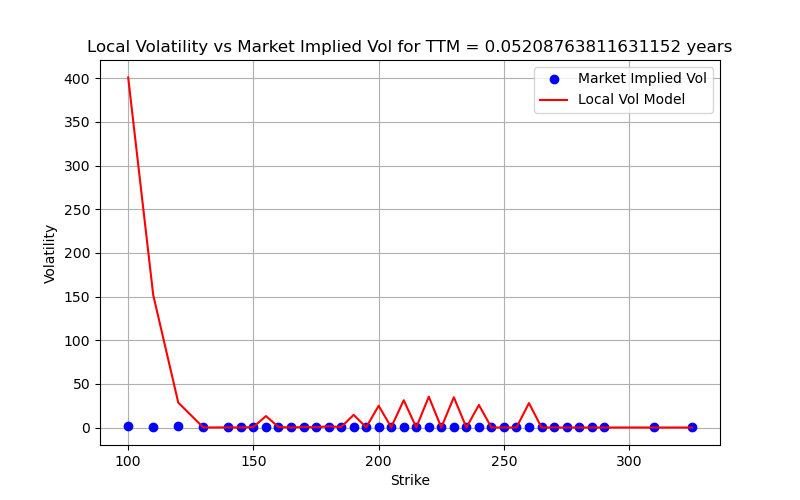
\includegraphics[width=1\textwidth]{bad_local_vol.png}
\caption{Local volatility calibration for short-term maturity.}
\label{fig:bad_local_vol}
\end{figure}

\begin{figure}[H]
\centering
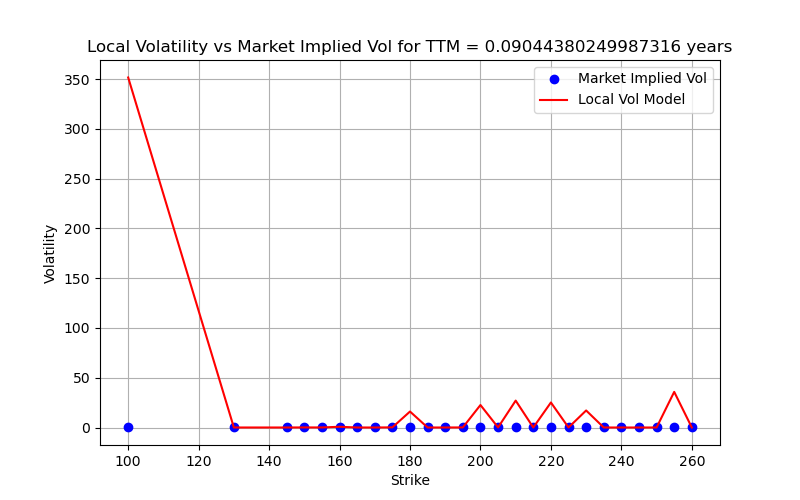
\includegraphics[width=1\textwidth]{bad_local_vol_2.png}
\caption{Local volatility calibration for another maturity.}
\label{fig:bad_local_vol_2}
\end{figure}


\subsubsection{Issues Observed in the Calibration}

The following problems are obvious:
\begin{itemize}
\item Extreme spikes in local volatility: The red curve (local volatility) shows unrealistic spikes, particularly for small strikes.
\item High instability for out-of-the-money (OTM) options: The local volatility values oscillate wildly at larger strikes.
\item Unrealistic values: Volatility values exceed reasonable market levels (e.g., 400\%+), which is not expected in practice.
\end{itemize}

\subsubsection{Potential Causes of Instability}
The observed issues can stem from several numerical and structural problems:
\begin{itemize}
\item \textbf{Noise in Implied Volatility and Market Prices}:
Implied volatility surfaces often exhibit noise due to market microstructure effects. Direct differentiation of noisy option prices amplifies errors, leading to extreme values in the local volatility calculation.

\item \textbf{Poor Estimation of Second Derivatives}:
The term $\frac{\partial^2 C}{\partial K^2}$ in the denominator is crucial. If this second derivative is small or poorly estimated, the formula will produce large and unstable values. Numerical differentiation on a sparse or irregular grid exacerbates this issue.

\item \textbf{Boundary Effects and Extrapolation Issues}:
Near the edges of the dataset (low or high strikes), extrapolation methods might introduce unrealistic behaviors. Ensuring convexity in the price surface is crucial for stability.
\end{itemize}


\subsubsection{Possible Solutions}
To improve the local volatility calibration, the following solutions are recommended:
\begin{itemize}
\item Apply Smoothing on Implied Volatility: Use a parametric model (e.g., SABR, SVI) or a smoothing technique (e.g., Gaussian process regression) to preprocess the implied volatility surface before computing derivatives.
\item Filter Out Unrealistic Local Volatility Values: Apply a cap on excessive local volatilities to prevent numerical explosions.
\end{itemize}

\section{SABR}
\subsection{SABR Model}

The SABR (Stochastic Alpha Beta Rho) model, introduced by Hagan et al. in 2002, is a \textbf{stochastic volatility} model widely used for pricing and risk-managing options, particularly in markets with pronounced volatility smiles or skews (e.g., interest rate derivatives and FX options). The SABR model is known for its ability to capture the dynamics of implied volatility and provide accurate pricing for European options.

\subsubsection{Hypotheses of the SABR Model}

The SABR model is based on the following key assumptions:
\begin{enumerate}
    \item \textbf{Stochastic Volatility}: The volatility of the underlying asset is stochastic and follows a separate stochastic process.
    \item \textbf{CEV (Constant Elasticity of Variance) Dynamics}: The underlying asset price follows a CEV process, which allows for flexible modeling of the asset's price dynamics.
    \item \textbf{Correlation Between Asset and Volatility}: The asset price and its volatility are correlated, which helps capture the volatility smile or skew.
    \item \textbf{No Arbitrage}: There are no arbitrage opportunities in the market.
    \item \textbf{Risk-Free Rate}: The risk-free interest rate is constant and known.
    \item \textbf{No Dividends}: The underlying asset does not pay dividends during the life of the option.
\end{enumerate}

\subsubsection{Dynamics of the SABR Model}

The SABR model describes the dynamics of the underlying asset price \( F_t \) (e.g., a forward price) and its stochastic volatility \( \alpha_t \) using the following system of stochastic differential equations (SDEs):
\[
dF_t = \alpha_t F_t^\beta \, dW_t^F
\]
\[
d\alpha_t = \nu \alpha_t \, dW_t^\alpha
\]
where:
\begin{itemize}
    \item \( F_t \): The forward price of the underlying asset at time \( t \).
    \item \( \alpha_t \): The stochastic volatility at time \( t \).
    \item \( \beta \): The elasticity parameter (\( 0 \leq \beta \leq 1 \)), which controls the shape of the forward price distribution.
    \item \( \nu \): The volatility of volatility (vol of vol), which controls the variability of the volatility process.
    \item \( W_t^F \) and \( W_t^\alpha \): Two correlated Wiener processes (Brownian motions) with correlation \( \rho \), i.e., \( dW_t^F \cdot dW_t^\alpha = \rho \, dt \).
\end{itemize}

The parameter \( \beta \) determines the distribution of the forward price:
\begin{itemize}
    \item \( \beta = 0 \): Normal SABR model (forward prices can become negative).
    \item \( \beta = 1 \): Lognormal SABR model (forward prices remain positive).
    \item \( 0 < \beta < 1 \): CEV dynamics (intermediate behavior).
\end{itemize}

\subsubsection{Implied Volatility Formula}

The SABR model provides an approximate closed-form formula for the implied volatility \( \sigma_{\text{imp}}(K, F) \) of a European option with strike \( K \) and forward price \( F \):
\[
\sigma_{\text{imp}}(K, F) = \frac{\alpha}{(F K)^{(1-\beta)/2} \left[ 1 + \frac{(1-\beta)^2}{24} \ln^2\left(\frac{F}{K}\right) + \frac{(1-\beta)^4}{1920} \ln^4\left(\frac{F}{K}\right) \right]} \cdot \frac{z}{\chi(z)}
\]
where:
\begin{itemize}
    \item \( z = \frac{\nu}{\alpha} (F K)^{(1-\beta)/2} \ln\left(\frac{F}{K}\right) \)
    \item \( \chi(z) = \ln\left( \frac{\sqrt{1 - 2 \rho z + z^2} + z - \rho}{1 - \rho} \right) \)
\end{itemize}
\vspace{0.5cm}

\subsection{Calibration and Implementation}
\begin{enumerate}
    \item \textbf{Collect Market Data}:
    We use market-implied volatilities of the stock AAPL from YFinance API for European options with different strikes \( K_i \) and maturities \( T_i \). We also need the risk-free rate associated with it (from Treasury Bills or 10Y US Bonds) and dividend yield in order to compute the forward price $F_t$
    \item \textbf{Define the Objective Function}:
    We then implement the objective function to compute the sum of squared differences between market-implied volatilities and SABR-implied volatilities:
    \[
    f(\Theta) = \sum_{i=1}^N \left( \sigma_{\text{market}}(K_i, T_i) - \sigma_{\text{SABR}}(K_i, T_i; \Theta) \right)^2
    \]
    Where \( \Theta = (\alpha, \beta, \rho, \nu) \) is the vector of SABR parameters.
    \item \textbf{Set Initial Guesses and Constraints}:
    We initial the parameters \( \Theta = (\alpha, \beta, \rho, \nu) \) and define the constraints:
    \begin{itemize}
        \item \( \alpha > 0 \)
        \item \( 0 \leq \beta \leq 1 \)
        \item \( -1 \leq \rho \leq 1 \)
        \item \( \nu > 0 \)
    \end{itemize}
    \item \textbf{Run the Optimization}:
    We then use an optimization algorithm (using Scipy) to minimize the objective function \( f(\Theta) \) and find the optimal parameter values.
    \end{enumerate}

The comparison between the SABR model-implied volatilities and market-implied volatilities is crucial for assessing the quality of the fit. Figures \ref{fig:sabr_calibration1} and \ref{fig:sabr_calibration2} present examples of volatility smiles for different times to maturity (TTM) before and after calibration. 

\newpage

\begin{figure}[h!]
    \centering
    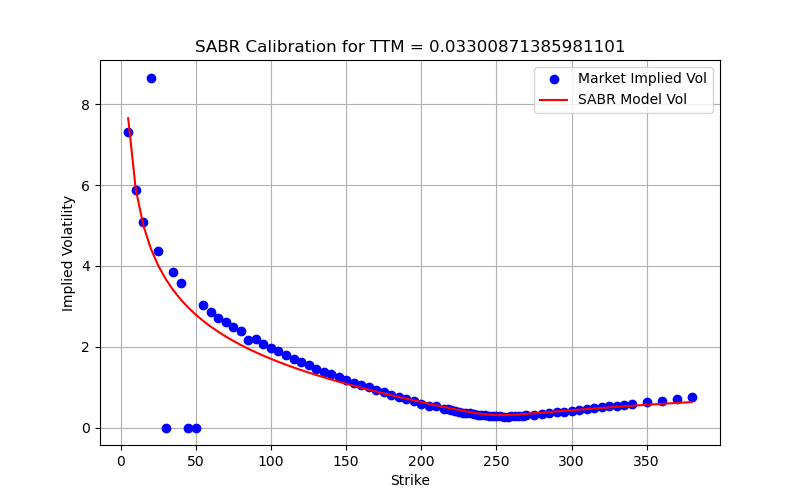
\includegraphics[width=1\textwidth]{Figure_1.png}
    \caption{SABR Calibration for Short-Term TTM (12 days to maturity)}
    \label{fig:sabr_calibration1}
\end{figure}

\begin{figure}[h!]
    \centering
    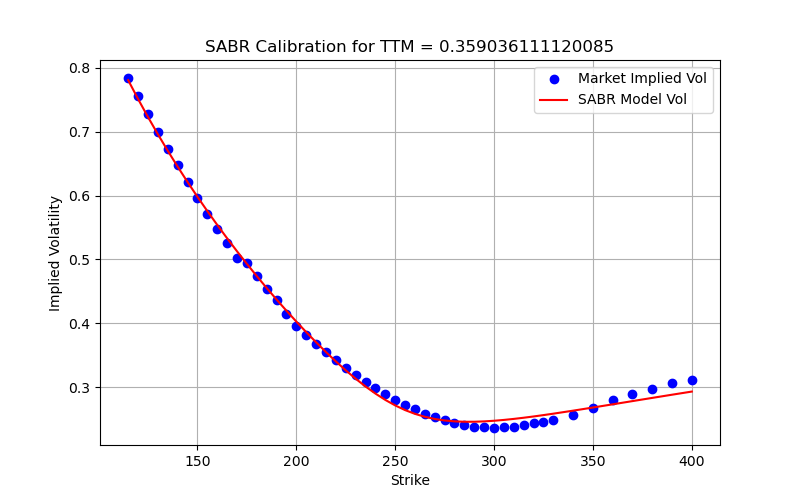
\includegraphics[width=1\textwidth]{sabr.png}
    \caption{SABR Calibration for Medium-Term TTM (131 days to maturity)}
    \label{fig:sabr_calibration2}
\end{figure}

The figures illustrate that the SABR model effectively captures the overall shape of the volatility smile, particularly in at-the-money and slightly out-of-the-money regions. However, there are notable limitations:

\begin{itemize}
    \item \textbf{Extreme Strikes:} At very low and high strikes, the model tends to diverge slightly from observed market volatilities. This is likely due to market microstructure effects and liquidity constraints, which are not explicitly accounted for in the model.
    \item \textbf{Short-Term Expirations:} The first figure (short TTM) shows that the SABR model struggles to capture sharp volatility spikes at lower strikes, which may indicate a need for an adjusted beta parameter or a stochastic volatility extension.
    \item \textbf{Low Volatility Environments:} The second figure (medium-term TTM) demonstrates a strong fit but highlights some deviations in deep out-of-the-money strikes. This suggests that the SABR model might require additional flexibility, such as skew adjustments or alternative volatility dynamics, to better fit market-implied volatilities.
\end{itemize}

Overall, while the SABR model is effective at modeling implied volatility, its assumptions —particularly the lognormality of returns and fixed correlation— can introduce some limitations. These limitations are more pronounced in extreme market conditions or for short-term maturities where volatility dynamics evolve rapidly.




% Chapter 2
\chapter{Systematic Trading Strategies}
\section{Introduction}
Systematic investment strategies use predefined rules to determine asset allocation and risk management. This report details the implementation of a trend-following strategy combined with factor-based selection, optimizing momentum and carry signals to enhance portfolio performance. This strategy is cross-asset and implies trading with 5 different indexes : SPY, EFA, IEF, VNQ and GSG. Additionally, a mean-reversion strategy on the Brent/WTI spread is examined.

\section{Asset Selection and Data Collection}
The selected asset universe comprises a diversified set of asset classes, retrieved from YFinance API in Python:
\begin{itemize}
    \item \textbf{Equities:} SPY (US equities), EFA (International equities)
    \item \textbf{Fixed Income:} IEF (US Treasuries)
    \item \textbf{Real Estate:} VNQ (Real estate investment trusts)
    \item \textbf{Commodities:} GSG (Broad commodity index), Brent Front Month (EU Crude oil), WTI Front Month (US Crude oil)
\end{itemize}
These assets were chosen for their distinct risk-return characteristics and diversification benefits.

\begin{figure}
    \centering
    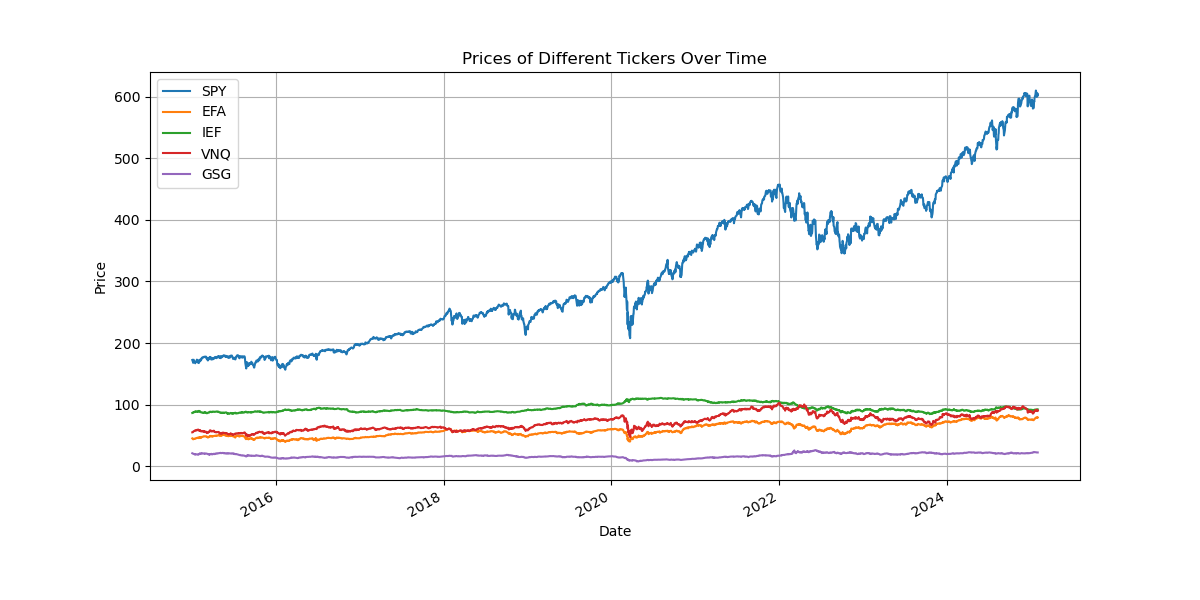
\includegraphics[width=1.1\textwidth]{asset_prices.png}
    \caption{Historical Price Evolution of SPY,EFA,IEF,VNQ,GSGG}
\end{figure}

\begin{figure}
    \centering
    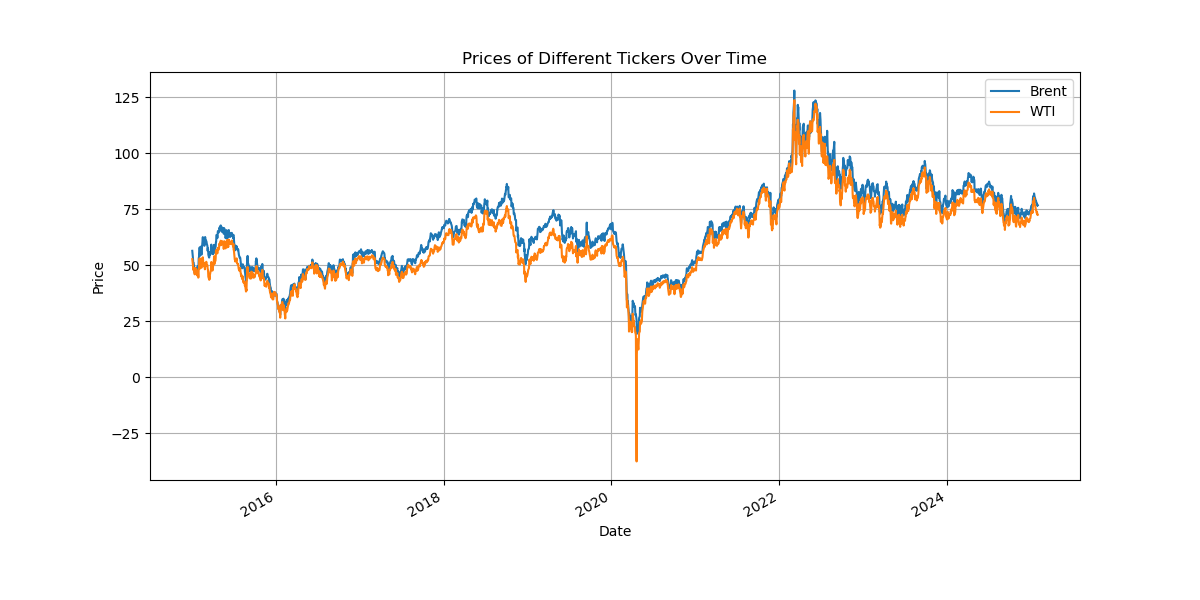
\includegraphics[width=1.1\textwidth]{wti_brent.png}
    \caption{Historical Price Evolution Brent and WTI Front month}
\end{figure}
\newpage


\section{Assumptions}
The strategies presented in this report rely on several key assumptions:
\begin{itemize}
    \item Market prices are efficient enough to allow systematic strategies to capture trends and mean-reverting behaviors.
    \item Fixed transaction costs (0.001 per price unit) .
    \item Asset price relationships, such as the Brent/WTI spread, exhibit mean-reverting tendencies over time.
    \item Selected assets provide sufficient liquidity for systematic trading without excessive market impact.
    \item The chosen lookback periods for trend and mean reversion calculations adequately reflect historical patterns.
\end{itemize}


\section{Trend Following Strategy}
Trend-following strategies rely on the principle that assets exhibiting upward momentum tend to continue their trajectory. This approach is implemented using a simple moving average (SMA) rule:
\begin{equation}
    SMA_t = \frac{1}{N} \sum_{i=0}^{N-1} P_{t-i}
\end{equation}
where $P_t$ is the asset price at time $t$ and $N$ is the SMA lookback period (set to 175 days in this study). An asset is considered to be in an \textbf{uptrend} if:
\begin{equation}
    P_t > SMA_t
\end{equation}

In that case, we should go \textbf{long} the asset, until the end of the signal.

\subsection{Momentum and Carry Factors}
Momentum is a key driver of asset returns, reflecting the tendency for past winners to outperform. We use 6-month and 12-month momentum signals:
\begin{equation}
    M_{6M,t} = \frac{P_t}{P_{t-126}} - 1, \quad M_{12M,t} = \frac{P_t}{P_{t-252}} - 1
\end{equation}
Carry is estimated using the rolling yield approach:
\begin{equation}
    C_t = \frac{\text{Rolling 21-day MA price}}{P_t}
\end{equation}

\subsection{Factor Combination and Ranking}
A normalized score is computed for each factor:
\begin{equation}
    Z_f = \frac{f_t - \mu_f}{\sigma_f}
\end{equation}
where $\mu_f$ and $\sigma_f$ are the mean and standard deviation of factor $f$ over the historical period.

The final ranking score is computed as:
\begin{equation}
    S_t = 0.5 M_{6M,t} + 0.5 M_{12M,t} + C_t
\end{equation}
Assets are ranked based on $S_t$, and only the top $N$ assets that are also in \textbf{uptrend} (see Section 2.4) are selected for allocation. By adjusting the parameter factor-weighting-method, we can decide to use only  $M_{6M,t}$ or $M_{12M,t}$ for the score, or any other combinations (see code-base).

\subsection{De-Risking Mechanism}
To mitigate excessive drawdowns, a rolling drawdown-based de-risking strategy is applied:
\begin{itemize}
    \item The portfolio’s rolling peak is computed over a 6-month window.
    \item The drawdown is measured as ($C_r$ is the cumulative return at time $r$):
    \begin{equation}
        DD_t = \frac{\max_{s \in [t-120,t]} C_s - C_t}{\max_{s \in [t-120,t]} C_s}
    \end{equation}
    \item If the drawdown exceeds a predefined threshold (e.g., 10\%), exposure is gradually reduced by a factor (e.g., 50\%) over multiple days.
\end{itemize}
This approach prevents excessive losses while allowing for partial participation in market recoveries.


\subsection{Grid Search for Hyperparameter Optimization}
To fine-tune the trend-following strategy, a grid search is employed to optimize key hyperparameters:
\begin{itemize}
    \item 	\textbf{SMA period:} The lookback period for the moving average (e.g., 100, 125, 150 days).
    \item 	\textbf{Momentum Type:} Evaluating different weighting schemes (6M vs. 12M momentum or combined momentum-carry factor).
    \item 	\textbf{Number of Selected Assets ($N$):} Choosing the optimal number of top-ranked assets for allocation (e.g., 3,2 or 5).
    \item 	\textbf{Rebalancing Frequency:} Testing weekly vs. monthly rebalancing to assess impact on performance and transaction costs.
\item \textbf{Allocation Method:} Comparing equal-weight vs. volatility-adjusted weighting.

\begin{itemize}
    \item \textbf{Equal-Weight Allocation:} Each asset or trading position receives the same weight, regardless of volatility or risk.
    \begin{equation}
        w_i = \frac{1}{N}
    \end{equation}
    where:
    \begin{itemize}
        \item $w_i$ is the weight of asset $i$,
        \item $N$ is the total number of assets or trades.
    \end{itemize}

    \item \textbf{Volatility-Adjusted Weighting:} Positions are sized inversely proportional to their historical volatility, ensuring more stable risk allocation.
    \begin{equation}
        w_i = \frac{\frac{1}{\sigma_i}}{\sum_{j=1}^{N} \frac{1}{\sigma_j}}
    \end{equation}
    where:
    \begin{itemize}
        \item $\sigma_i$ is the historical realized volatility (e.g., using a 20-day rolling window) of asset $i$,
        \item $w_i$ is the normalized weight ensuring the sum of weights equals 1.
    \end{itemize}
\end{itemize}
    \item 	\textbf{Max Drawdown over 6 months:} Maximum drawdown threshold for de-risking mechanism.
    \item 	\textbf{Reduce exposure:} Proportion of reduced exposure.

\end{itemize}
Each combination of parameters is tested in the backtest framework, and the optimal set is selected based on maximizing the Sharpe ratio while minimizing drawdowns. 

\subsection{Backtest Results}
The strategy is backtested over a 10-year period (from 01/01/2015 to 01/02/2025), starting with a capital at 100 000 dollars. We use those indexes as our assets for the strategy : SPY, EFA, IEF, VNQ and GSG. We evaluate : Cumulative returns, Sharpe Ratio and Maximum Drawdown. The hyper-parameters used are (cf Section 2.4.4) :
\begin{itemize}
    \item 	\textbf{SMA period:} 175
    \item 	\textbf{Momentum Type:} Momentum 12M (e.g, the score function is $S_t$ = $M_{12M,t}$)
    \item 	\textbf{Number of Selected Assets :} 2
    \item 	\textbf{Rebalancing Frequency:} Weekly.
    \item 	\textbf{Allocation Method:} volatility-adjusted weighting.
    \item 	\textbf{Max Drawdown over 6 months:} 0.1.
    \item 	\textbf{Reduce exposure:} 0.5.
\end{itemize}



\subsection{Performance Analysis}

The trend-following strategy significantly outperformed the static equal-weighted benchmark:
\begin{itemize}
    \item Total Net Return: 170.95\% vs. 79.96\% (benchmark)
    \item Sharpe Ratio: 1.02 vs. 0.53
    \item Maximum Drawdown: 16.26\% vs. 28.28\%
\end{itemize}

\begin{figure}[H]
    \centering
    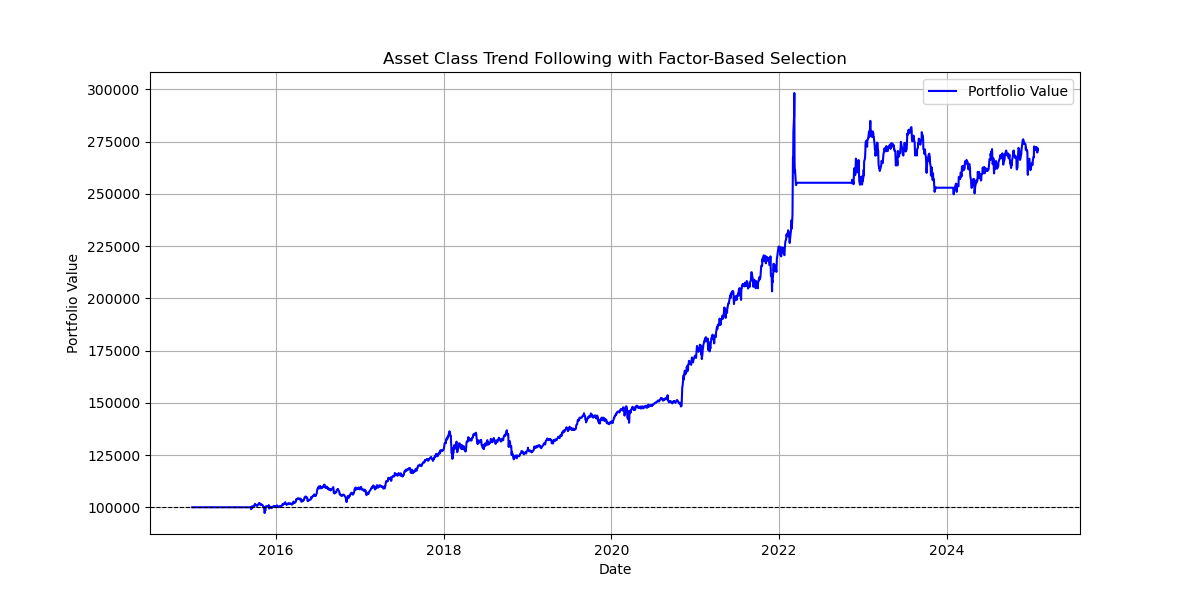
\includegraphics[width=1.2\textwidth]{asset_trend_post_cost.png}
    \caption{Cumulative Returns of the Trend Strategy}
\end{figure}

\begin{figure}[H]
    \centering
    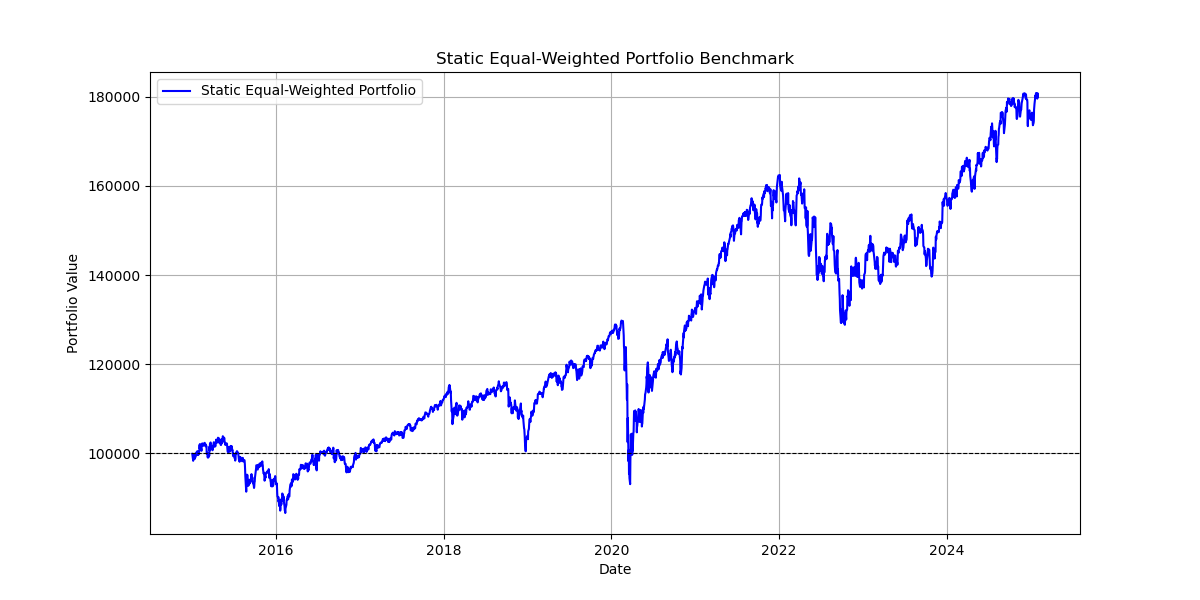
\includegraphics[width=1.2\textwidth]{asset_trend_benchmark.png}
    \caption{Cumulative Returns of the benchmark (equally-weighted portfolio on the 5 indexes)}
\end{figure}


The trend-following strategy not only delivered higher returns, but also exhibited better risk-adjusted performance and lower drawdowns, suggesting that dynamic asset selection and de-risking contributed to superior capital preservation.
\\
\\
Despite its strong performance, the strategy has some limitations:

\begin{itemize}
    \item High Sensitivity to Transaction Costs: Weekly rebalancing increases turnover, potentially eroding net returns when trading costs are high.
    \item Sector Concentration Risks: A sharp portfolio value increase in 2022 coincides with strong commodity performance, highlighting exposure to sectoral trends. This could lead to over-reliance on specific market conditions.
    \item Lag in Market Regime Changes: Trend-following strategies react with a lag, making them vulnerable to sudden market reversals where short-term volatility dominates.
\end{itemize}

Overall, the strategy demonstrates strong return generation with controlled risk, outperforming a static allocation. However, transaction cost efficiency and exposure diversification remain key areas for optimization in future research.


\section{Mean Reversion Strategy on Brent/WTI Spread}
Mean-reversion strategies rely on the assumption that asset spreads revert to their historical mean. We use the spread between Brent and WTI crude oil prices, defining it as:
\begin{equation}
    Spread_t = P_{Brent, t} - P_{WTI, t}
\end{equation}
A rolling mean and standard deviation are computed to define a normalized Z-score:
\begin{equation}
    Z_t = \frac{Spread_t - \mu_{Spread}}{\sigma_{Spread}}
\end{equation}
A position is taken when:
\begin{itemize}
    \item $Z_t < -2$: Long the spread (buy Brent, sell WTI)
    \item $Z_t > 2$: Short the spread (sell Brent, buy WTI)
    \item $-0.5 < Z_t < 0.5$: Close the position
\end{itemize}
To avoid extreme deviations, a safeguard is introduced:
\begin{equation}
    \text{Extreme Condition} = |Spread_t| > |\mu_{Spread} + 1.5 \times \sigma_{Spread}|
\end{equation}
where positions are not entered if the spread is in an extreme condition.


\subsection{Backtest Results and Performance Analysis}
The strategy is backtested over a 10-year period (from 01/01/2015 to 01/02/2025), starting with a capital at 100 000 dollars.
The mean reversion strategy based on the Brent/WTI spread showed stable but lower returns:

\begin{itemize}
    \item Total Net Return: 40.02\%
    \item Sharpe Ratio: 0.42
    \item Maximum Drawdown: 11.85\%
\end{itemize}

\newpage

\begin{figure}
    \centering
    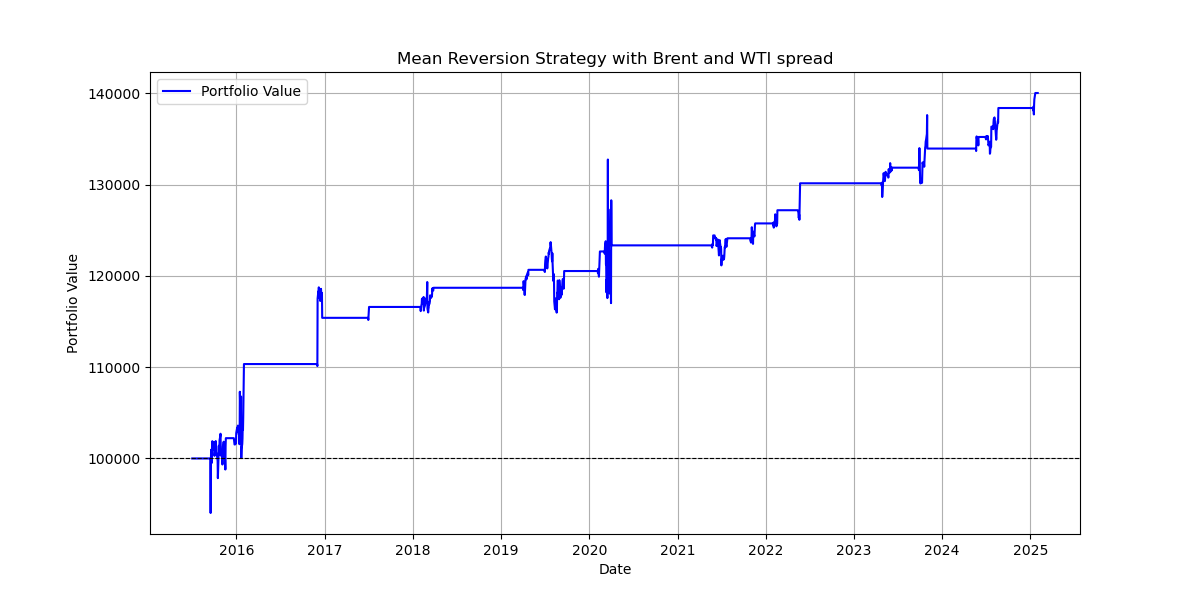
\includegraphics[width=1.2\textwidth]{wti_brent_spread.png}
    \caption{Cumulative Returns of the Strategies}
\end{figure}

This strategy exhibited lower volatility and smaller drawdowns, making it a more conservative approach. However, it also has notable limitations:

\begin{itemize}
    \item Limited Profit Potential: Mean reversion strategies tend to generate smaller returns compared to trend-following strategies.
    \item Sensitivity to Spread Behavior: The profitability depends on the stability of the Brent/WTI spread reverting to its historical mean.
\end{itemize}


\chapter{Conclusion}
The second part details two systematic strategies: trend-following with factor-based selection cross-asset (5 indexes fund) and a mean-reversion strategy on the Brent/WTI spread. The combination of these approaches allows for diversified risk-adjusted returns. Future research could refine and blend the two strategies within a portfolio, this could lead to general improve of Sharpe Ratio and performance.

\end{document}

